\chapter{Server}
Der Webserver ist unter 193.175.199.115 erreichbar:

\begin{itemize}
\item StudMap.Admin: \href{http://193.175.199.115/StudMapAdmin}{http://193.175.199.115/StudMapAdmin}
\item StudMap.Client: \href{http://193.175.199.115/StudMapClient}{http://193.175.199.115/StudMapClient}
\item StudMap.Service: \href{http://193.175.199.115/StudMapService}{http://193.175.199.115/StudMapService}
\end{itemize}


\section{Software}
Auf dem Server sind folgende Softwarekomponenten installiert:
\begin{itemize}
\item Internet Information Services (Version 7.5)
\item Microsoft SQL Server 2012
\end{itemize}

\section{Einrichtung IIS}

\begin{wrapfigure}{r}{0.4\textwidth}
\vspace{-20pt}
  \begin{center}
    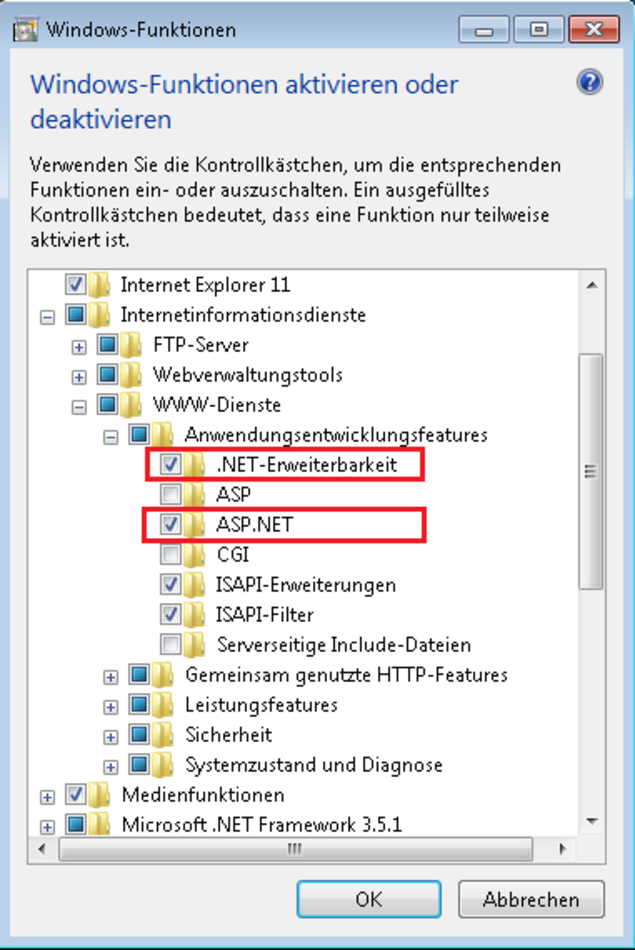
\includegraphics[width=0.9\linewidth]{../Bilder/Install_IIS}
  \end{center}
  \vspace{-20pt}
\end{wrapfigure}

Der IIS kann sowohl auf einem Windows Server als auch auf einer normalen Windows Installation eingerichtet werden. Dazu w�hlt man unter "`Programme"' > "`Windows-Features installieren oder deinstallieren"' aus. Daraufhin �ffnet sich ein Dialog (s. Abbildung), indem der IIS zur Installation ausgew�hlt werden kann.

Nach Abschluss der Installation steht der IIS-Manager zur Verf�gung und Webseiten k�nnen eingerichtet werden. 

Da auf unserem Server kein Serverbetriebssystem, sondern lediglich ein Standard Windows 
installiert ist, steht "`Web Deploy"' nicht zur Verf�gung. Daher m�ssen Deployment Pakete
manuell erstellt und auf dem Server aufgespielt werden. Dazu klickt man in Visual Studio 
auf den Kontextmen�punkt "`Ver�ffentlichen"' des jeweiligen Projektes. Anschlie�end kann
das Deployment Package im IIS �ber einen Rechtsklick auf "`StudMap"'>"'Bereitstellen"'>"'Anwendung importieren"' 
importiert werden.

\section{Einrichtung SQL Server}
Im Projekt wird ein Microsoft SQL Server 2012 verwendet. Da unsere Anwendung 
auf komplexe Managementfunktionen verzichtet kann auch die kostenlose Express 
Version genutzt werden.

Der Aufbau der Datenbank kann aus dem im SVN eingecheckten  
\href{https://studmap.googlecode.com/svn/database/StudMapDBSkript.sql}{Datenbankskripten} hergestellt werden.
